\documentclass[11pt, a4paper]{article}		% general format


%%%% Charset
\usepackage[utf8]{inputenc}					% use utf8					
\usepackage[russian]{babel}					% use russian font


%%%% Math
\usepackage{amsmath}						% Amer­i­can Math­e­mat­i­cal So­ci­ety (AMS) math fa­cil­i­ties
\usepackage{amsfonts}						% fonts from the AMS
\usepackage{amssymb}						% additional math symbols


%%%% Graphics
\usepackage{graphicx}


\author{Бусаров Владислав}
\title{Отчет по лабораторной работе №6 :\\ Набор инструментов для аудита беспроводных сетей AirCrack}
\date{2015}

%---------------------------------------------------------

\begin{document}
\maketitle
\tableofcontents
\newpage

%---------------------------------------------------------


\section{Цель работы}

Изучить основные возможности пакета AirCrack и принципы взлома WPA/WPA2 PSK и WEP.



%---------------------------------------------------------

\section{Ход работы}


%---------------------------------------------------------

\subsection{Изучить документацию по основным утилитам пакета – airmon-ng, airodump-ng, aireplay-ng, aircrack-ng.}

Aircrack-ng - набор программ, предназначенных для обнаружения беспроводных сетей, перехвата передаваемого через беспроводные сети трафика, аудита WEP и WPAWPA2-PSK ключей шифрования (проверка стойкости), в том числе пентеста (Penetration test) беспроводных сетей (подверженность атакам на оборудование и атакам на алгоритмы шифрования).

Программа работает с любыми беспроводными сетевыми адаптерами, драйвер которых поддерживает режим мониторинга (список можно найти на сайте программы). Программа работает в операционных системах Windows, UNIX, Linux и Mac OS X. 

Версия для UNIX-подобных операционных систем имеет значительно бьшую функциональность и поддерживает больше беспроводных адаптеров, чем Windows-версия. aircrack-ng был также портирован для платформ Zaurus и Maemo. Также программа была портирована для iPhone.

airmon-ng	Выставления различных карт в режим мониторинга.

aireplay-ng	Пакетный инжектор (Linux и Windows).

aircrack-ng	Взламывает ключи WEP и WPA (Перебор по словарю).



%---------------------------------------------------------

\subsection{Запустить режим мониторинга на беспроводном интерфейсе}

airmon-ng start wlan0mon

\begin{verbatim}
Found 3 processes that could cause trouble.
If airodump-ng, aireplay-ng or airtun-ng stops working after
a short period of time, you may want to kill (some of) them!
-e 
PID	Name
2221	NetworkManager
3392	wpa_supplicant
7009	dhclient


Interface	Chipset		Driver

wlan0mon	Unknown 	rtl8192cu - [phy0]
(monitor mode enabled on [phy0]wlan0mon)

\end{verbatim}

%---------------------------------------------------------

\subsection{Запустить утилиту airodump, изучить формат вывода этой утили-ты, форматы файлов, которые она может создавать}

Запуск утилиты airodump:

airodump-ng wlan0mon

\begin{figure}[h!]
	\centering
	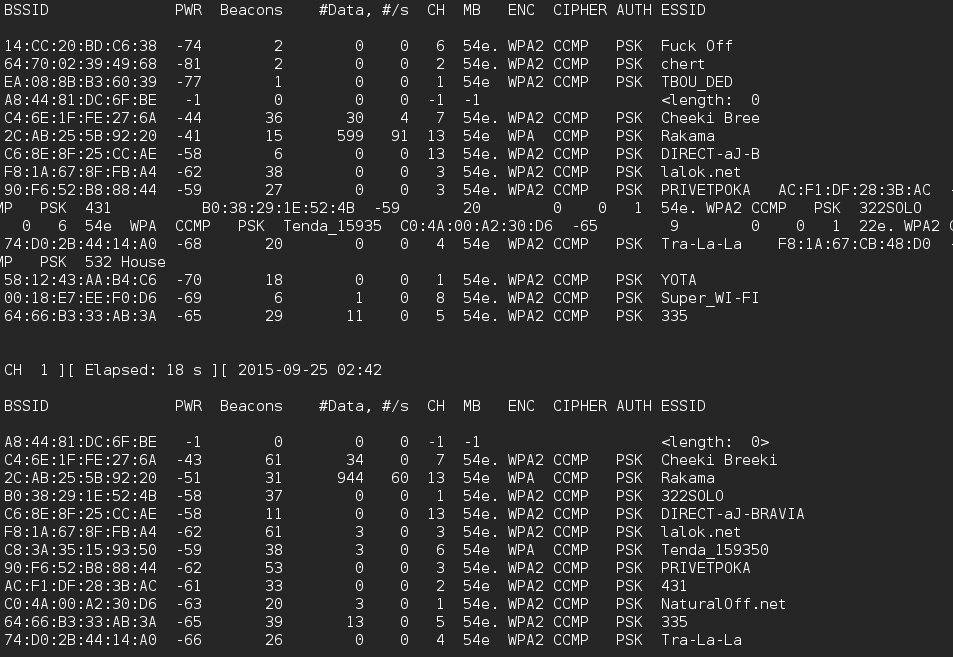
\includegraphics[scale=0.60]{res/2}
	\caption{Запуск airomon-ng}
\end{figure}

При указании ключа --write, утилита создает набор файлов с заданным префиксом. Два из которых связаны с информацией о доступных сетях и представлены в двух форматах: csv и xml. Еще два фала содержать информацию о перехваченных пакетах. Файл типа .cap содержит перехваченные пакеты, в то время как csv содержит лишь сокращенную информацию. Стоит отметить, что csv - это формат хранения простой таблицы.

cap - можно открыть в дальнейшем через wireshark, в нем отображаются все пакеты.




%---------------------------------------------------------

\subsection{Запустить сбор трафика для получения аутентификационных сообщений}

airodump-ng wlan0mon -w new1 --bssid C4:6E:1F:FE:27:6A 
Так же можно указать канал используя ключ: --channel

\begin{figure}[h!]
	\centering
	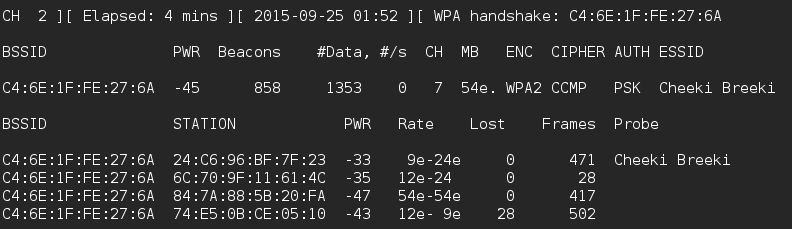
\includegraphics[scale=0.60]{res/3}
	\caption{Запуск airodump-ng}
\end{figure}


%---------------------------------------------------------

\subsection{Произвести деаутентификацию одного из клиентов, до тех пор, пока не удастся собрать необходимых для взлома аутенти-фикационных сообщений}

\begin{figure}[h!]
	\centering
	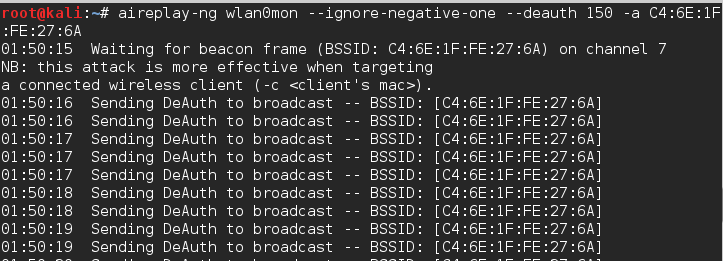
\includegraphics[scale=0.60]{res/4}
	\caption{DeAuth Broadcast}
\end{figure}


В результате перехватываем пакет handshake:

\begin{figure}[h!]
	\centering
	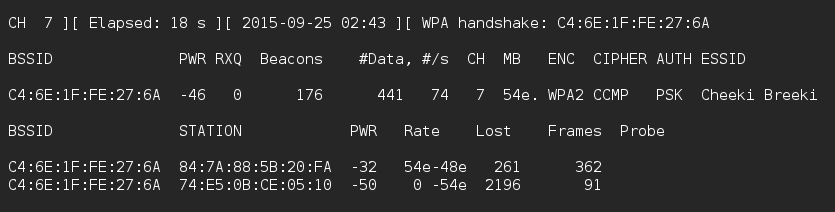
\includegraphics[scale=0.60]{res/5}
	\caption{airodump-ng Handshake}
\end{figure}

%---------------------------------------------------------

\subsection{Произвести взлом используя словарь паролей}

Так как используемый пароль слишком сложный, в некоторую часть словаря был вставлен искомый пароль.
Команда: aircrack-ng -w /tmp/words.lst -b C4:6E:1F:FE:27:6A /tmp/wpa2*.cap
words.lst - файл с предполагаемыми паролями. Это может быть какой-либо сборник слов или же обычный словарь.
wpa2.cap - файл airodump-ng который мы записали когда получили Handshake.
\begin{figure}[h!]
	\centering
	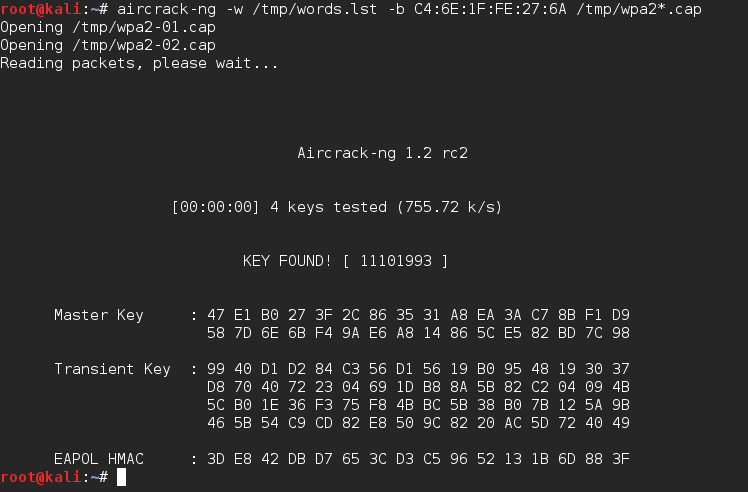
\includegraphics[scale=0.60]{res/6}
	\caption{Работа Aircrack-ng}
\end{figure}


%---------------------------------------------------------

\section{Выводы}

В ходе данной лабораторной работы был рассмотрен AirCrack с такими его уилитами, как: airmon-ng, airodump-ng, aireplay-ng и aircrack-ng.
 
Произведен мониоринг на беспроводном инерфейсе, ослеживающий аутентификации в сети, а также осуществлена деаутентификация одного из клиентов и перехвачен введенный им пароль. В итоге осуществден взлом, посредсвом словаря паролей.



\end{document}